\documentclass{article}
\usepackage{tikz}
\usetikzlibrary{arrows.meta}

\begin{document}

\begin{figure}[h]
    \centering
    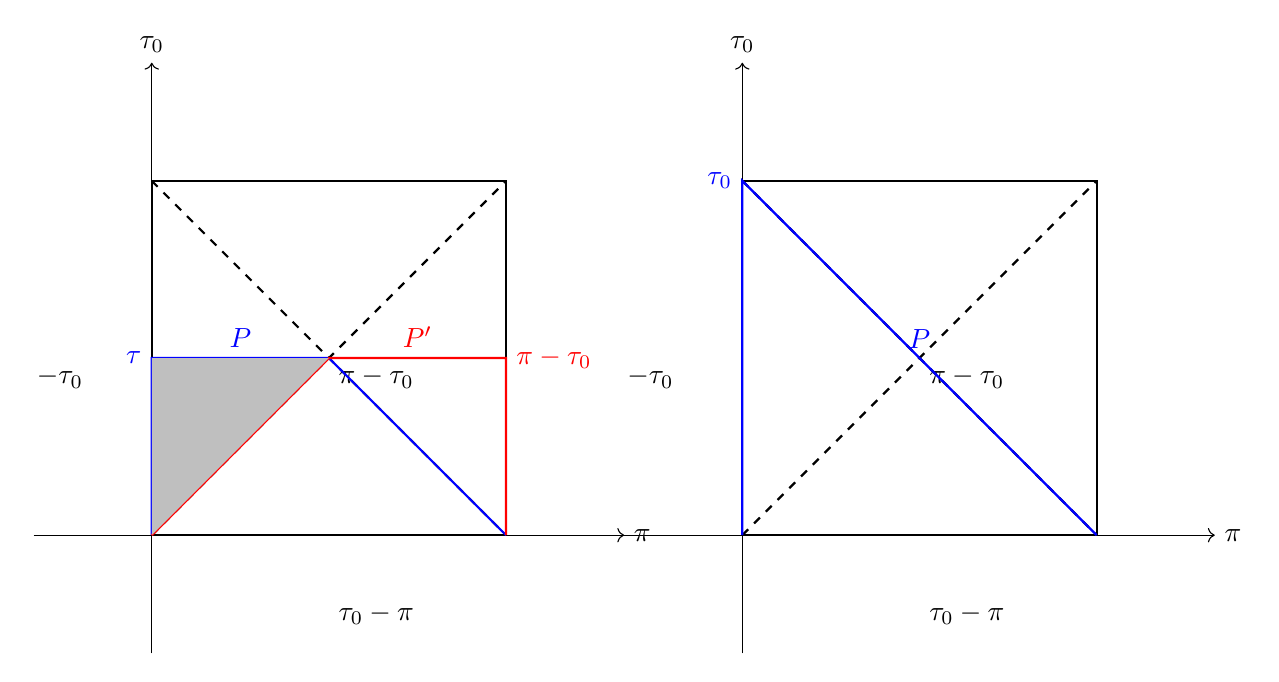
\begin{tikzpicture}[scale=1.5]
        % Draw the coordinate system
        \draw[->] (-1,0) -- (4,0) node[right] {$\pi$};
        \draw[->] (0,-1) -- (0,4) node[above] {$\tau_0$};
        
        % Draw the Penrose diagram
        \draw[thick] (0,0) rectangle (3,3);
        \draw[thick, dashed] (0,0) -- (3,3);
        \draw[thick, dashed] (0,3) -- (3,0);
        
        % Label the regions
        \node at (1.5, 1.5) [below right] {$\pi - \tau_0$};
        \node at (1.5, -0.5) [below right] {$\tau_0 - \pi$};
        \node at (-0.5, 1.5) [below left] {$-\tau_0$};
        
        % Draw the observer's patch P
        \draw[blue, thick] (0,0) -- (0,1.5) node[left] {$\tau$} -- (1.5,1.5) node[midway, above, blue] {$P$} -- (3,0);
        
        % Draw the complementary patch P'
        \draw[red, thick] (3,0) -- (3,1.5) node[right] {$\pi - \tau_0$} -- (1.5,1.5) node[midway, above, red] {$P'$} -- (0,0);
        
        % Shade the timelike envelope
        \fill[gray!50] (0,0) -- (0,1.5) -- (1.5,1.5) -- cycle;
        
        % Right panel
        \begin{scope}[xshift=5cm]
            % Draw the coordinate system
            \draw[->] (-1,0) -- (4,0) node[right] {$\pi$};
            \draw[->] (0,-1) -- (0,4) node[above] {$\tau_0$};
            
            % Draw the Penrose diagram
            \draw[thick] (0,0) rectangle (3,3);
            \draw[thick, dashed] (0,0) -- (3,3);
            \draw[thick, dashed] (0,3) -- (3,0);
            
            % Label the regions
            \node at (1.5, 1.5) [below right] {$\pi - \tau_0$};
            \node at (1.5, -0.5) [below right] {$\tau_0 - \pi$};
            \node at (-0.5, 1.5) [below left] {$-\tau_0$};
            
            % Draw the observer's patch P
            \draw[blue, thick] (0,0) -- (0,3) node[left] {$\tau_0$} -- (3,0);
            \node at (1.5, 1.5) [above, blue] {$P$};
        \end{scope}
    \end{tikzpicture}
    
    \caption{
        On the left panel, we depict the Penrose diagram for the case with $\pi/2 < \tau_0 < \pi$ where $P$ denotes the observer's patch at $\theta=0$ and $P'$ its complementary patch. The shaded region describes the timelike envelope of an observer from $\tau$ to $\tau_0$. On the right, we depict the case with $\tau_0 > \pi$ where the observer at $\theta=0$ can see the entire Cauchy slice.
    }
\end{figure}

\end{document}